\section{TADIP}
\label{sec:algorithms:tadip}

\begin{figure}[H]
    \centering
    \begin{subfigure}[b]{0.5\textwidth}
        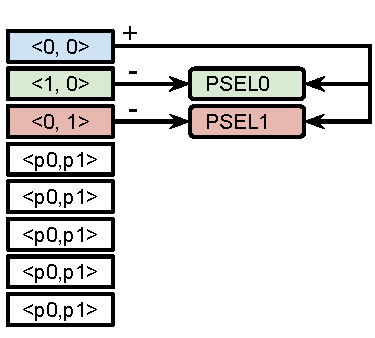
\includegraphics[width=\textwidth]{figures/algorithms/TADIP-I}
        \caption{Cache managed by TADIP-Isolated.}
        \label{fig:algorithms:tadip:isolated}
    \end{subfigure}
    \begin{subfigure}[b]{0.5\textwidth}
        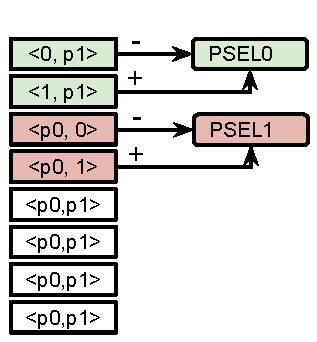
\includegraphics[width=\textwidth]{figures/algorithms/TADIP-F}
        \caption{Cache managed by TADIP-Feedback.}
        \label{fig:algorithms:tadip:feedback}
    \end{subfigure}    
    \caption{Two alternate duel set organizations for TADIP.}
    \label{fig:algorithms:tadip}
\end{figure}

Thread Aware Dynamic Insertion Policy (TADIP)~\cite{Jaleel2008} proposed by A. Jaleel et al. in 2008 is a thread-aware extension of DIP~\cite{Qureshi2007}.
The main issue with DIP that TADIP counters, is that DIP does not consider from which core a cache accesses originate.
In a workload with multiple benchmarks, some might be recency-friendly while others are not. 
If a shared cache is managed by DIP, then the algorithm choice is made based on the sum of the cache accesses and then applied equally to all benchmarks.
The authors of TADIP recognized that improvements in performance could be achieved by selecting the DIP policy on a per-core basis when utilized in a shared cache.

When selecting the best performing algorithm per core, the ATD technique requires two ATDs per core sharing the cache. 
This solution can quickly become too expensive to be practical.
Set-dueling in DIP requires a minimum of two sets, one running LRU (1) and one running BIP (0). 
With two cores, the number of combinations rises to four (00, 01, 10, 11).
When the number of cores increases this also seems to be an impractical solution.
As a result, the authors of TADIP suggests two selection techniques based on set dueling, but that reduces the number of duel sets required.
Both solutions have one saturating counter per core sharing the cache.
This counter is used to select the optimal policy for that core.

TADIP-Isolated (TADIP-I) has one set per core running BIP for that core and LRU for all others.
In addition to these N sets, a single set runs LRU for all cores. 
A miss in the LRU set will increment all the core counters while a miss in the core specific set will decrement the counter for the specific core.
For a large N, this solution requires significantly less duel-sets compared to having one per combination ($N+1 << N^2$). 
This solution assumes that all other cores run LRU, and, therefore, cannot fully capture the effect of interactions between cores.
Figure~\ref{fig:algorithms:tadip:isolated} shows an example of a cache managed by TADIP-I. 
In the figure, PSEL0 is the saturating counter used to select the optimal policy for core 0.
Within a set $<0, 0>$ indicates that both cores run LIP while $<1, 0>$ indicates that core 0 runs BIP while core 1 runs LIP.
The variables p0 and p1 represent the current optimal policy for core 0 and 1 respectively.

TADIP-Feeback (TADIP-F) attempts to reduce the error caused by the assumption of other cores by having two sets per core, a total of 2N.
A cache managed by TADIP-F is illustrated in figure~\ref{fig:algorithms:tadip:feedback}.
Per core, one set runs LRU the other runs BIP, any inserts from other cores uses the currently best algorithm for that core.
Like in the other policies, a miss in the LRU set for a core will increment that cores counter and a miss the BIP set will decrement the counter.
For the remainder of this thesis when we refer to TADIP we assume TADIP-F unless otherwise stated.

When implementing TADIP, some mechanism is required to select which sets are duel sets, and which are follower sets.
The authors of TADIP provides a simple hash function that can be used to select dueling sets, shown in algorithm~\ref{alg:algorithms:tadip:set_selection}.
On their 4096 set cache, they use the formulas shown below.
In the algorithm, set index is a number from 0-4095, core\_id is the zero-indexed id of the requester core and cores is the total number of cores sharing the cache.
If BIP or LIP is true, then the set is a duel set for the given core, and the policy forced to either BIP or LIP.
If both BIP and LIP is false, then the set is a normal follower set and utilizes the current best algorithm for the given core.
From the algorithm, it is clear that the original authors use a total of 32 groups of duel sets spread evenly throughout the cache.
\begin{algorithm}[ht]
\begin{equation}
LIP = set\_no[11:7] + core\_id == set\_no[6:0]
\end{equation}
\begin{equation}
BIP = set\_no[11:7] + core\_id + cores == set\_no[6:0]
\end{equation}
\begin{equation}
FOLLOWER = !LIP + !BIP
\end{equation}
\label{alg:algorithms:tadip:set_selection}
\caption{TADIP duel set selection}
\end{algorithm}
